\section{The complete survivable embedded virtual network embedding algorithm}
In this section, we first present the procedure of added resource allocation  for virtual network with survivable guarantee.
%, then we also give out resource demand allocation method fitting for both FD-SeVN and FI-SeVN embedding, since the difference between FD-SeVN and FI-SeVN in embedding approach could be reconciled by a general resources sharing constraint.
More details would be elaborated in the following part.

Besides, with respect to the node mapping even and virtual link mapping, because not all the virtual links or not all their bandwidth would be employed simultaneously under single one node failure, some virtual links could share physical resources if they are embedded on the same physical link, which would reduce the total needed physical bandwidth. In short, backup bandwidth of physical link corresponding different virtual network request edge could be shared each other.


\subsection{Embed Added Backup Resource into physical network}
From Sec.\ref{lab:DynamicProgrammingEquation}, we have obtained node mapping relationship with respect to node $v_i$ failure, and compute out how much computation of every node should to be reallocated  and how much bandwidth of every link should to be reallocate  in physical network $G(S,L)$ as shown in Fig.\ref{fig:AugmentResource}. Added computation resource 0,2,0,0,3,6,0 in physical node $s_1,s_2,s_3,s_4,s_5,s_6,s_7$, respectively. Finding five path with bandwidth 1,4,6,3,6 corresponding to physical path $p_{s_1s_2},p_{s_1s_3},p_{s_1s_5},p_{s_1s_6},p_{s_2s_5}$, respectively. Even though there were most virtual network embedding algorithms, node mapping phase had been completed with respect to our algorithm, the next procedure describing edge mapping phase. We use standard shortest path algorithm-dijkstra algorithm\cite{skiena1990dijkstra} to request added path of physical node , and reallocate some bandwidth to these paths of physical network for this virtual network survivable request. some research\cite{yu2008rethinking} focus on path embedding and path split embedding in order to achieve high link utilization, link stress and other objective target, but we do not focus the edge mapping problem in the paper.

\begin{figure}
  \centering
  % Requires \usepackage{graphicx}
  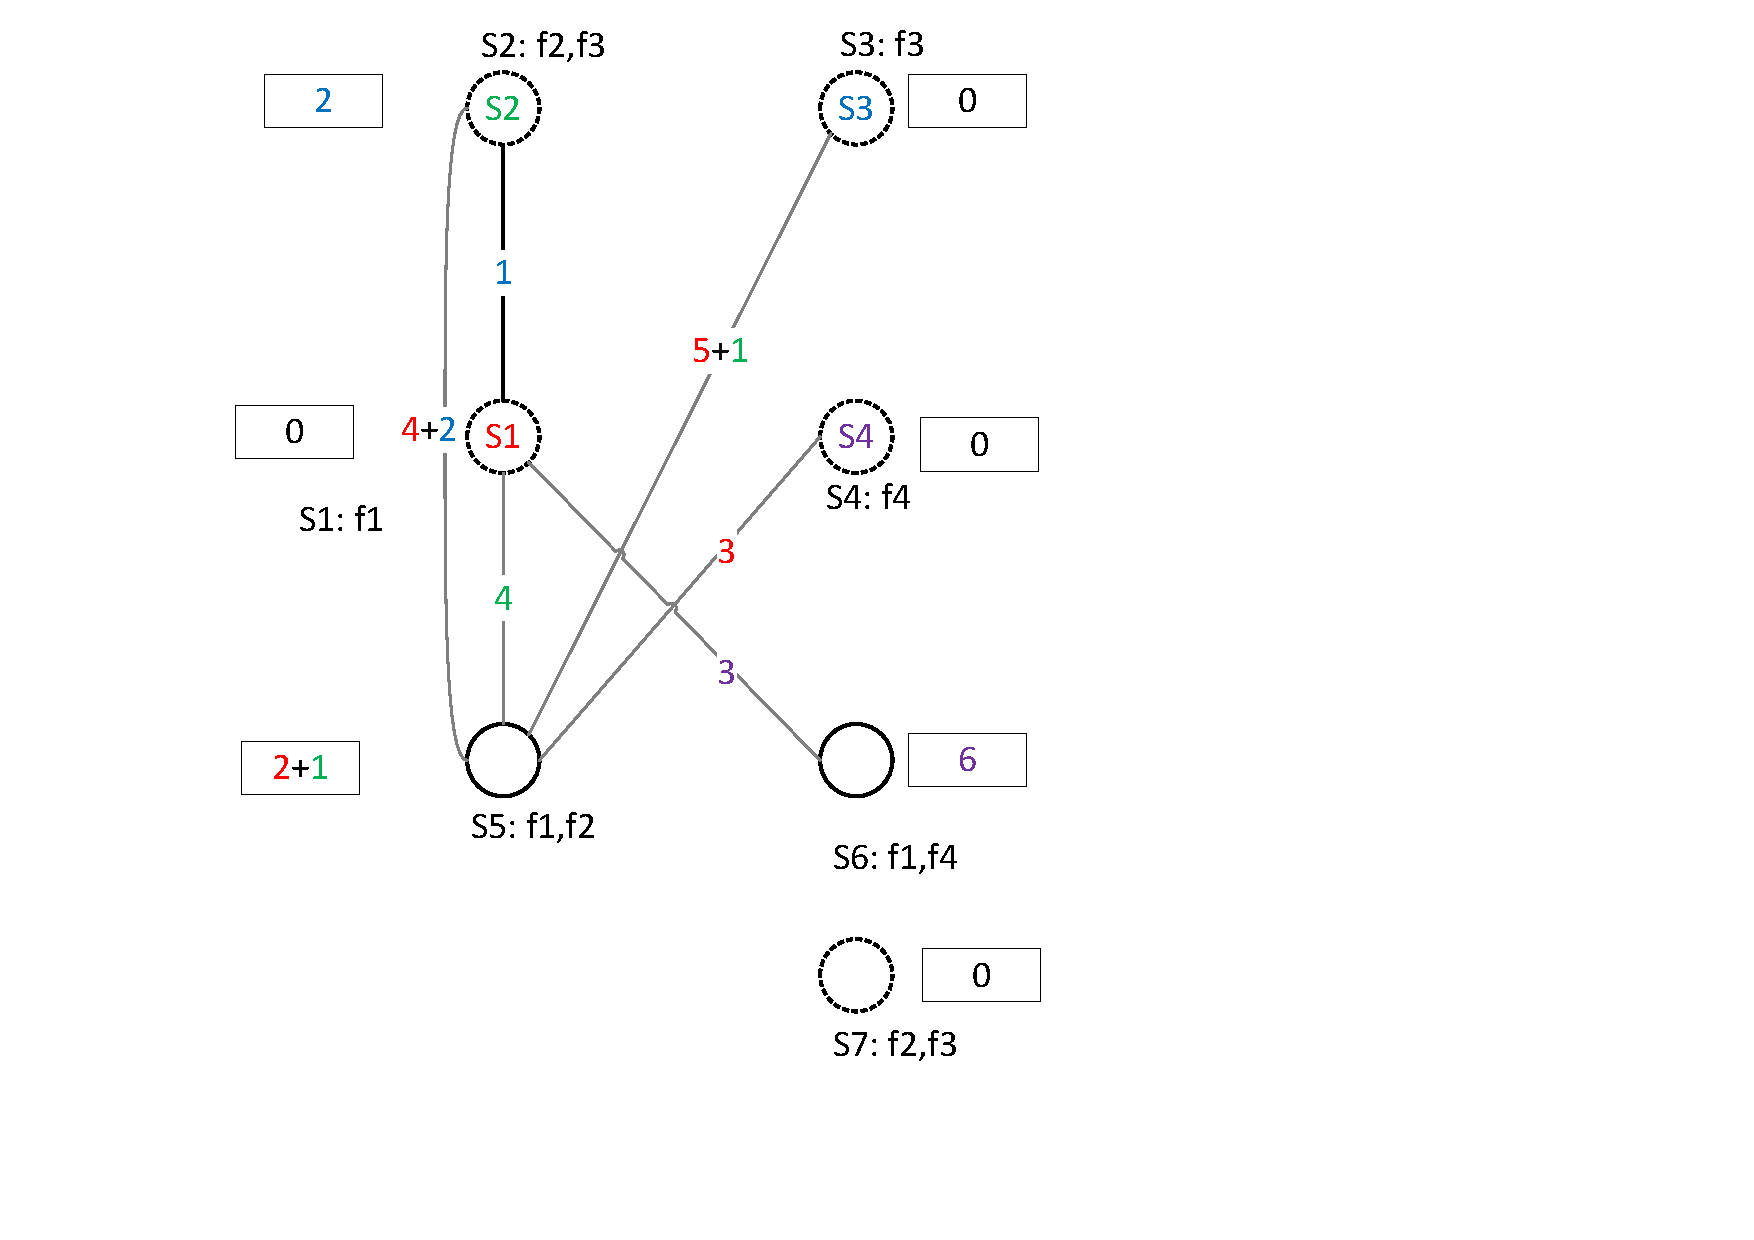
\includegraphics[width=2in]{Fig/AugmentResource}\\
  \caption{Added backup resource}\label{fig:AugmentResource}
\end{figure}

Finally, we iteratively repeat the procedure of graph decomposition iand multiple knapsack problem in Sec.\ref{lab:Graphdecompositionbasedproblemformulation} for following each physical node embedded virtual node failure to re-construct the added graph for guaranteeing virtual network survivable request. As shown in Fig.\ref{fig:Node4Failure}, partial added resource which is labeled consecutively with different color of the physical network illustrate each node failure is presented consecutively. It is worth noting that, every step of partial added physical resource is based on the previous step of added physical resource.

\subsection{Algorithm procedure}
In this section, we describe out complete algorithm procedure of survivable virtual network embedding problem as shown in Alg.\ref{alg:SeVNAlg}
\begin{algorithm}[htbp]
\label{alg:SeVNAlg}
\caption{survivable embedded virtual network algorithm}
\begin{algorithmic}[1]
\REQUIRE $G (V,E)$: virtual network's request; $G (S,L)$: physical network .
\ENSURE Generate SeVN and embed SeVN added resource into physical network.
\STATE Embed Virtual Network $G(V,E)$ into Physical Network $G(S,L)$\cite{liu2011completing}.
\STATE Extract embedded virtual network eVN $G\left( {\hat S,\hat L} \right)$ from physical network corresponding to this VN embedding request
%\STATE AllMinimumCycle($G(V,E)$)
\FORALL{$v_i$ such that $v_i\in V$}
\STATE Decompose eVN $G\left( {\hat S,\hat L} \right)$ into two star structure sets $VS(i)$ and $PS(j)$ from graph $G\left( {\hat S,\hat L} \right)$.
\STATE Construct items based star structure set $VS(i)$.
\STATE Construct knapsacks based star structure set $PS(j)$ from embedded virtual network eVN.
\STATE Construct edge cost matrix based in (\ref{eq:edge weight}) or (\ref{eq:new edge weight}).
\STATE Solve multiple knapsack problem through dynamic programming in Sec.\ref{lab:DynamicProgrammingEquation}.
\STATE Add new nodes, connect new edges, re-allocate node computing and edge's bandwidth into $G\left( {\hat S,\hat L} \right)$ to construct new graph $G\left( {\hat S,\hat L} \right)$.
\ENDFOR
\STATE Embed added resource or startup new nodes from SeVN $G\left( {\hat S,\hat L} \right)$ into physical network $G(S,L)$
\end{algorithmic}
\end{algorithm}

%1 node+2 node computaion+12 bandwidth
%0 node+1 node computaion+5 bandwidth
%1 node+5 node computaion+11 bandwidth
%1 node+6 node computaion+3 bandwidth
%=3 node+14 node computaion+31 bandwidth
%
%1 node+2 node computaion+12 bandwidth
%0 node+1 node computaion+5 bandwidth
%0 node+2 node computaion+3 bandwidth
%1 node+6 node computaion+3 bandwidth
%=2 node+11 node computaion+23 bandwidth
